\documentclass[tikz]{standalone}
\usepackage{graphicx}
\usepackage{subcaption}
\usepackage{caption}
\usepackage{comment}
\usepackage{tikz}
\usepackage{textcomp}

\definecolor{Okabe1}{RGB}{000,158,115}
\definecolor{Okabe2}{RGB}{000,114,178}
\definecolor{Okabe3}{RGB}{086,180,233}
\definecolor{Okabe4}{RGB}{230,159,000}
\definecolor{Okabe5}{RGB}{213,094,000}
\definecolor{Okabe6}{RGB}{204,121,167}

\definecolor{b1}{HTML}{d73027}
\definecolor{b2}{HTML}{fc8d59}
\definecolor{b3}{HTML}{ffffbf}
\definecolor{b4}{HTML}{91bfdb}
\definecolor{b5}{HTML}{4575b4}

\begin{document}
	\begin{comment}
		\begin{tabular}{@{}c@{}c@{}}
			\includegraphics[width=0.5\textwidth]{shellAmbient.jpg} &
			\includegraphics[width=0.5\textwidth]{shellCrushed.jpg} \\
			\noalign{\vskip -4pt}
			\includegraphics[width=0.5\textwidth]{shellNeg.jpg} &
			\includegraphics[width=0.5\textwidth]{shellHold.jpg}
		\end{tabular}.
	\end{comment}
	\begin{tikzpicture}
		\tikzstyle{every node}=[font=\LARGE]
		
		\node [anchor=south west] at (-1,5.5) {\color{black}{$b.$}};
		
		\node[anchor=south west,inner sep=0] at (0,0) {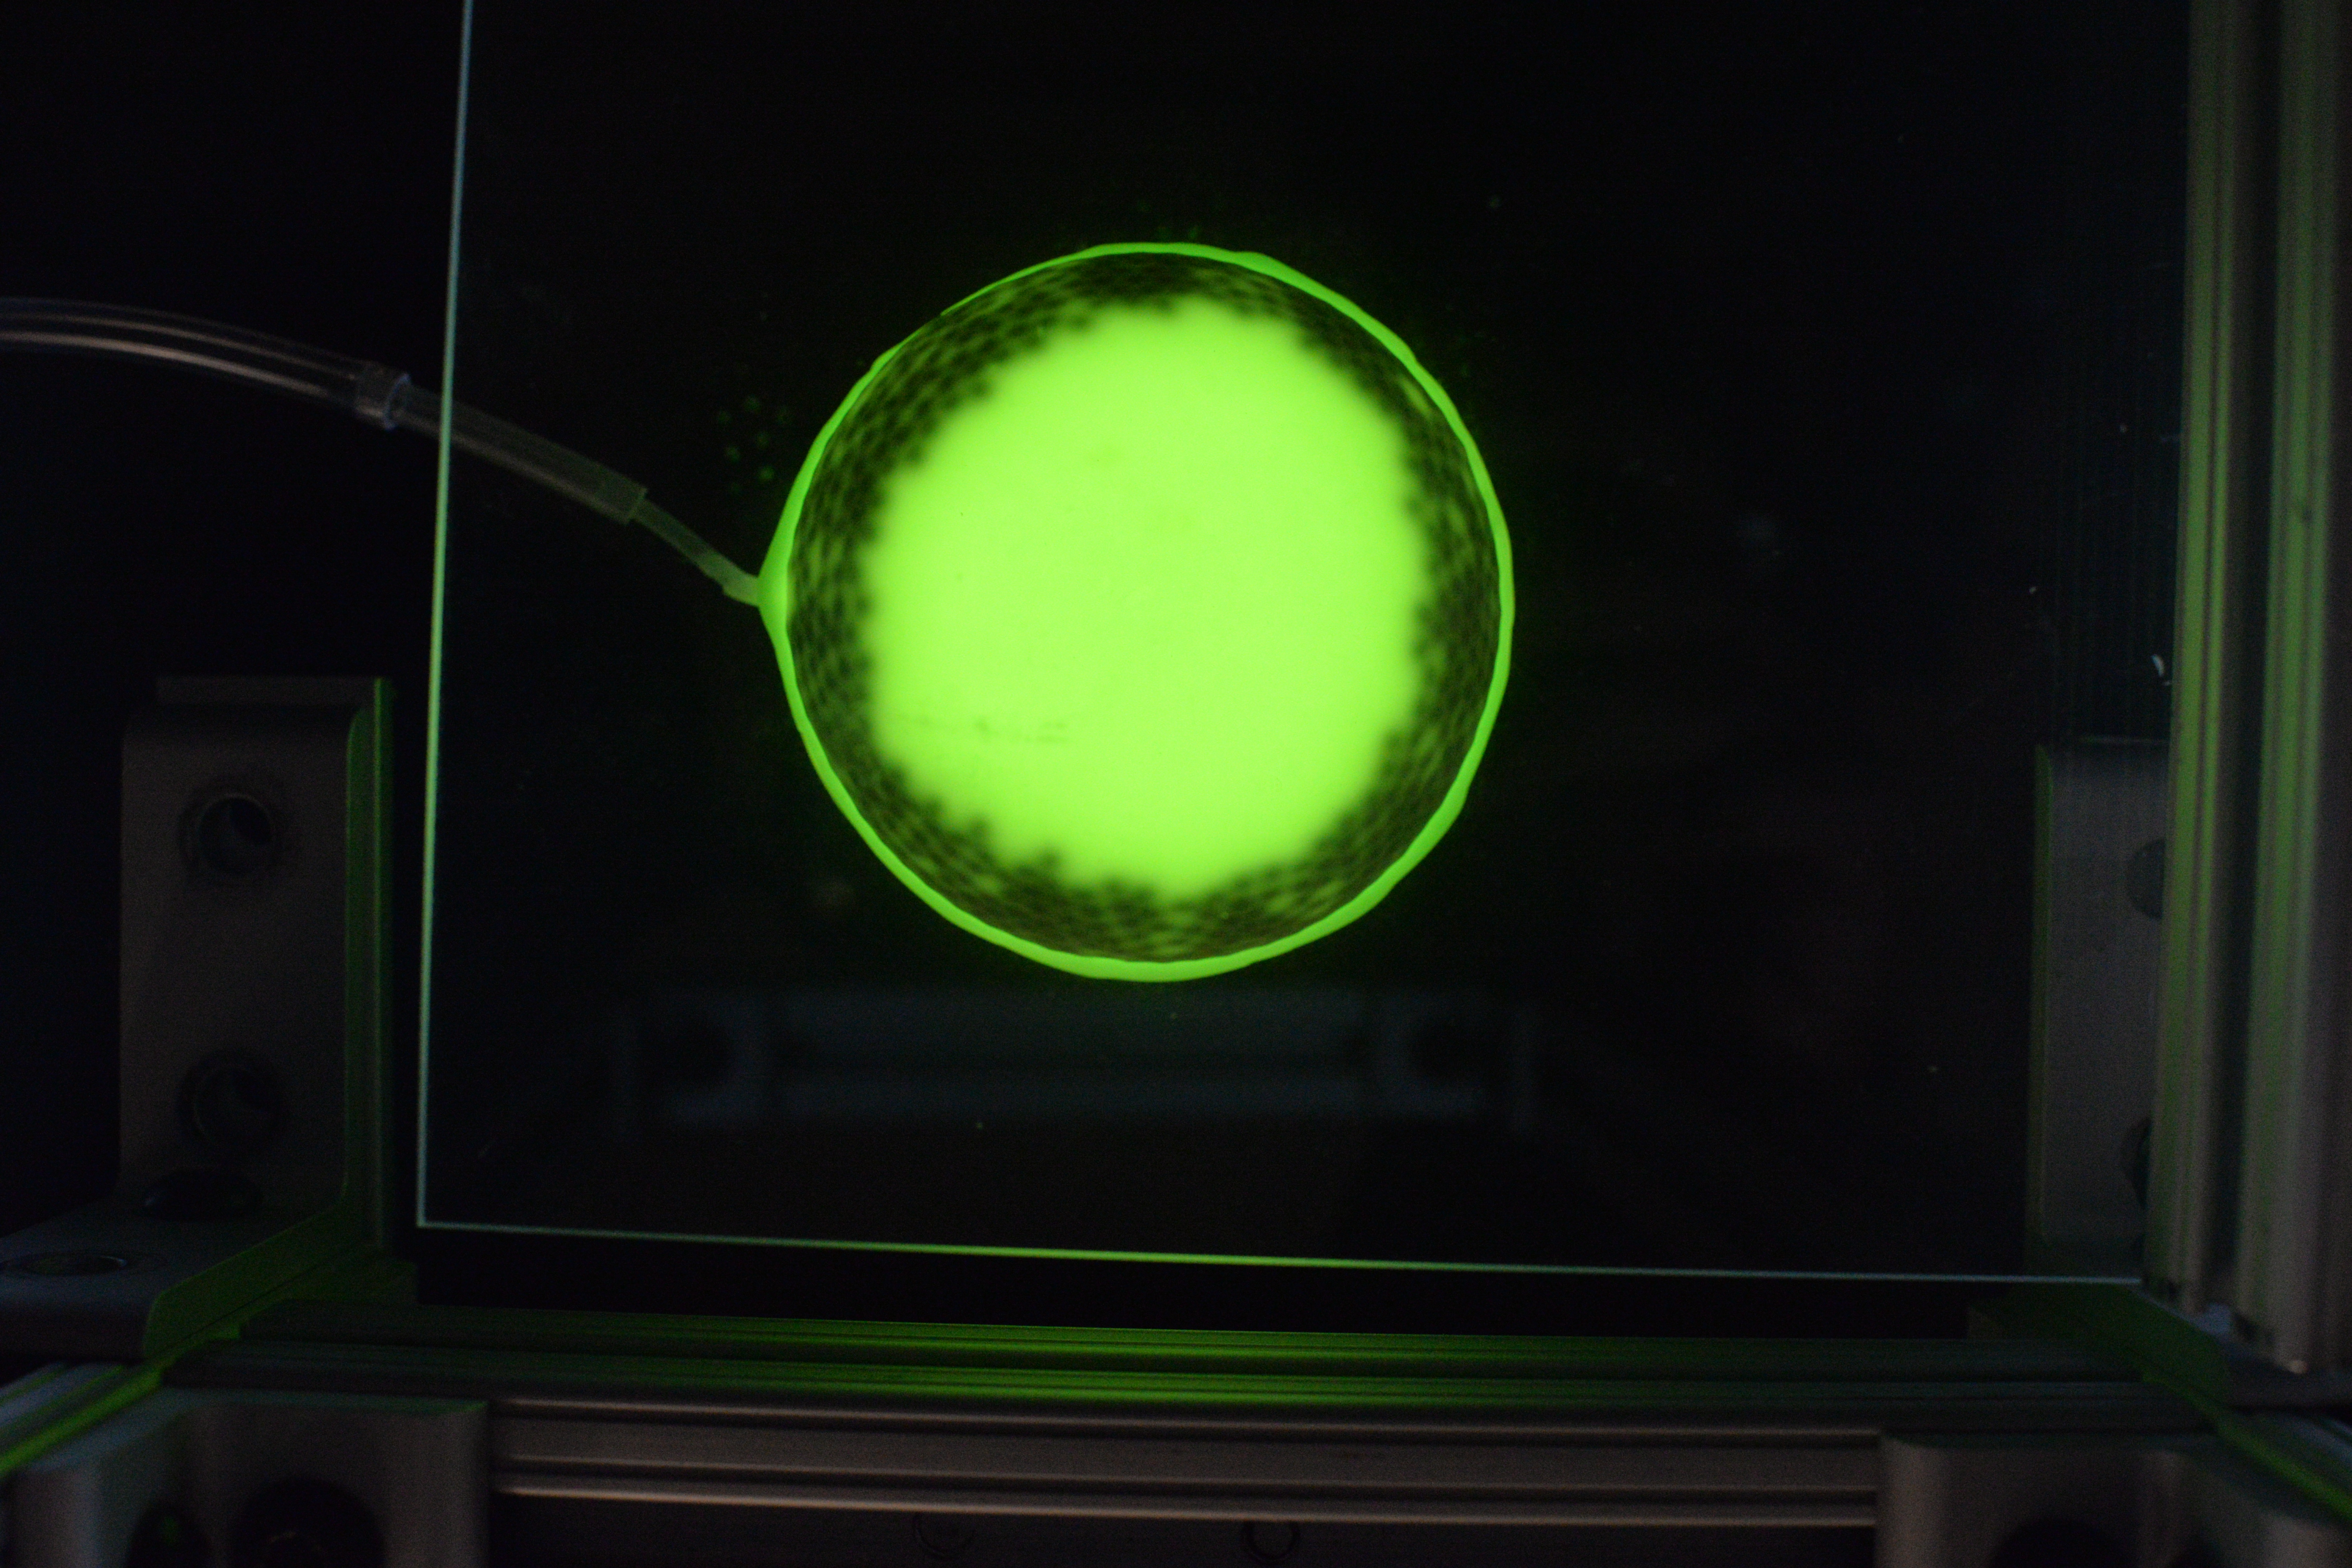
\includegraphics[trim = 335 250 370 95, clip, width=5cm,]{0.423-edge}};
		\node[anchor=south west,inner sep=0] at (5,0) {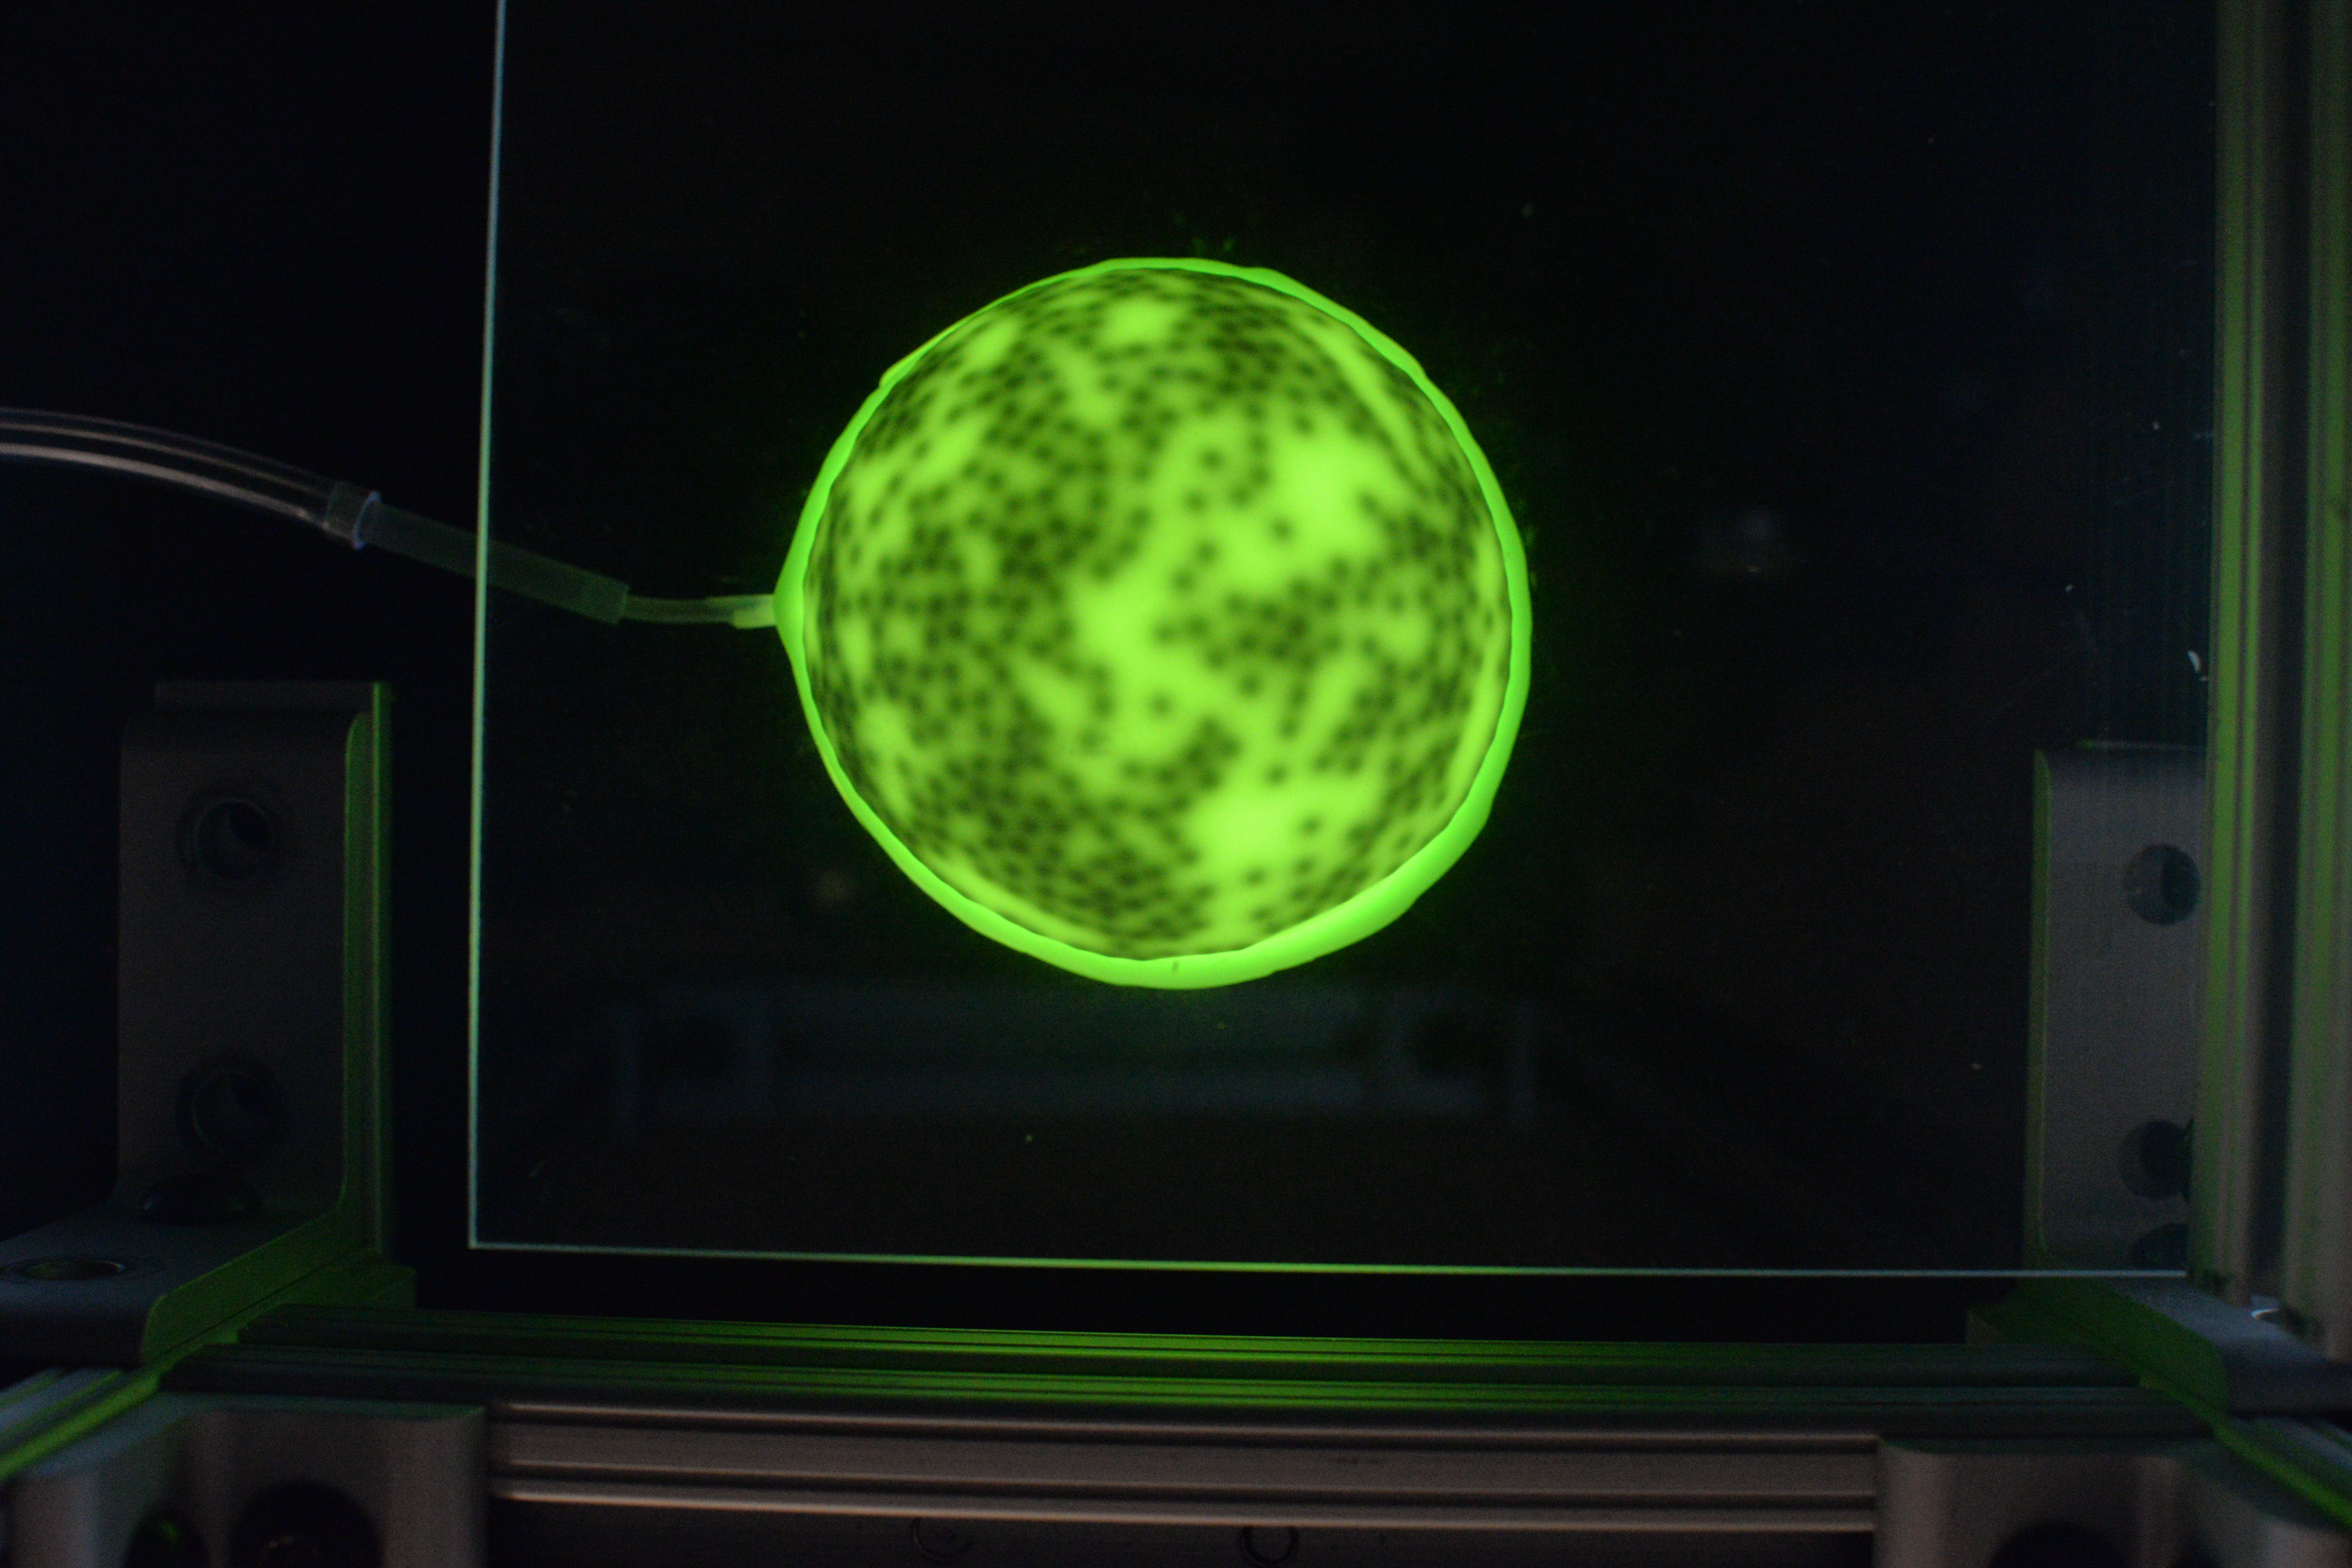
\includegraphics[trim = 345 250 360 95, clip, width=5cm]{0.423}};
		\node[anchor=south west,inner sep=0] at (10,0) {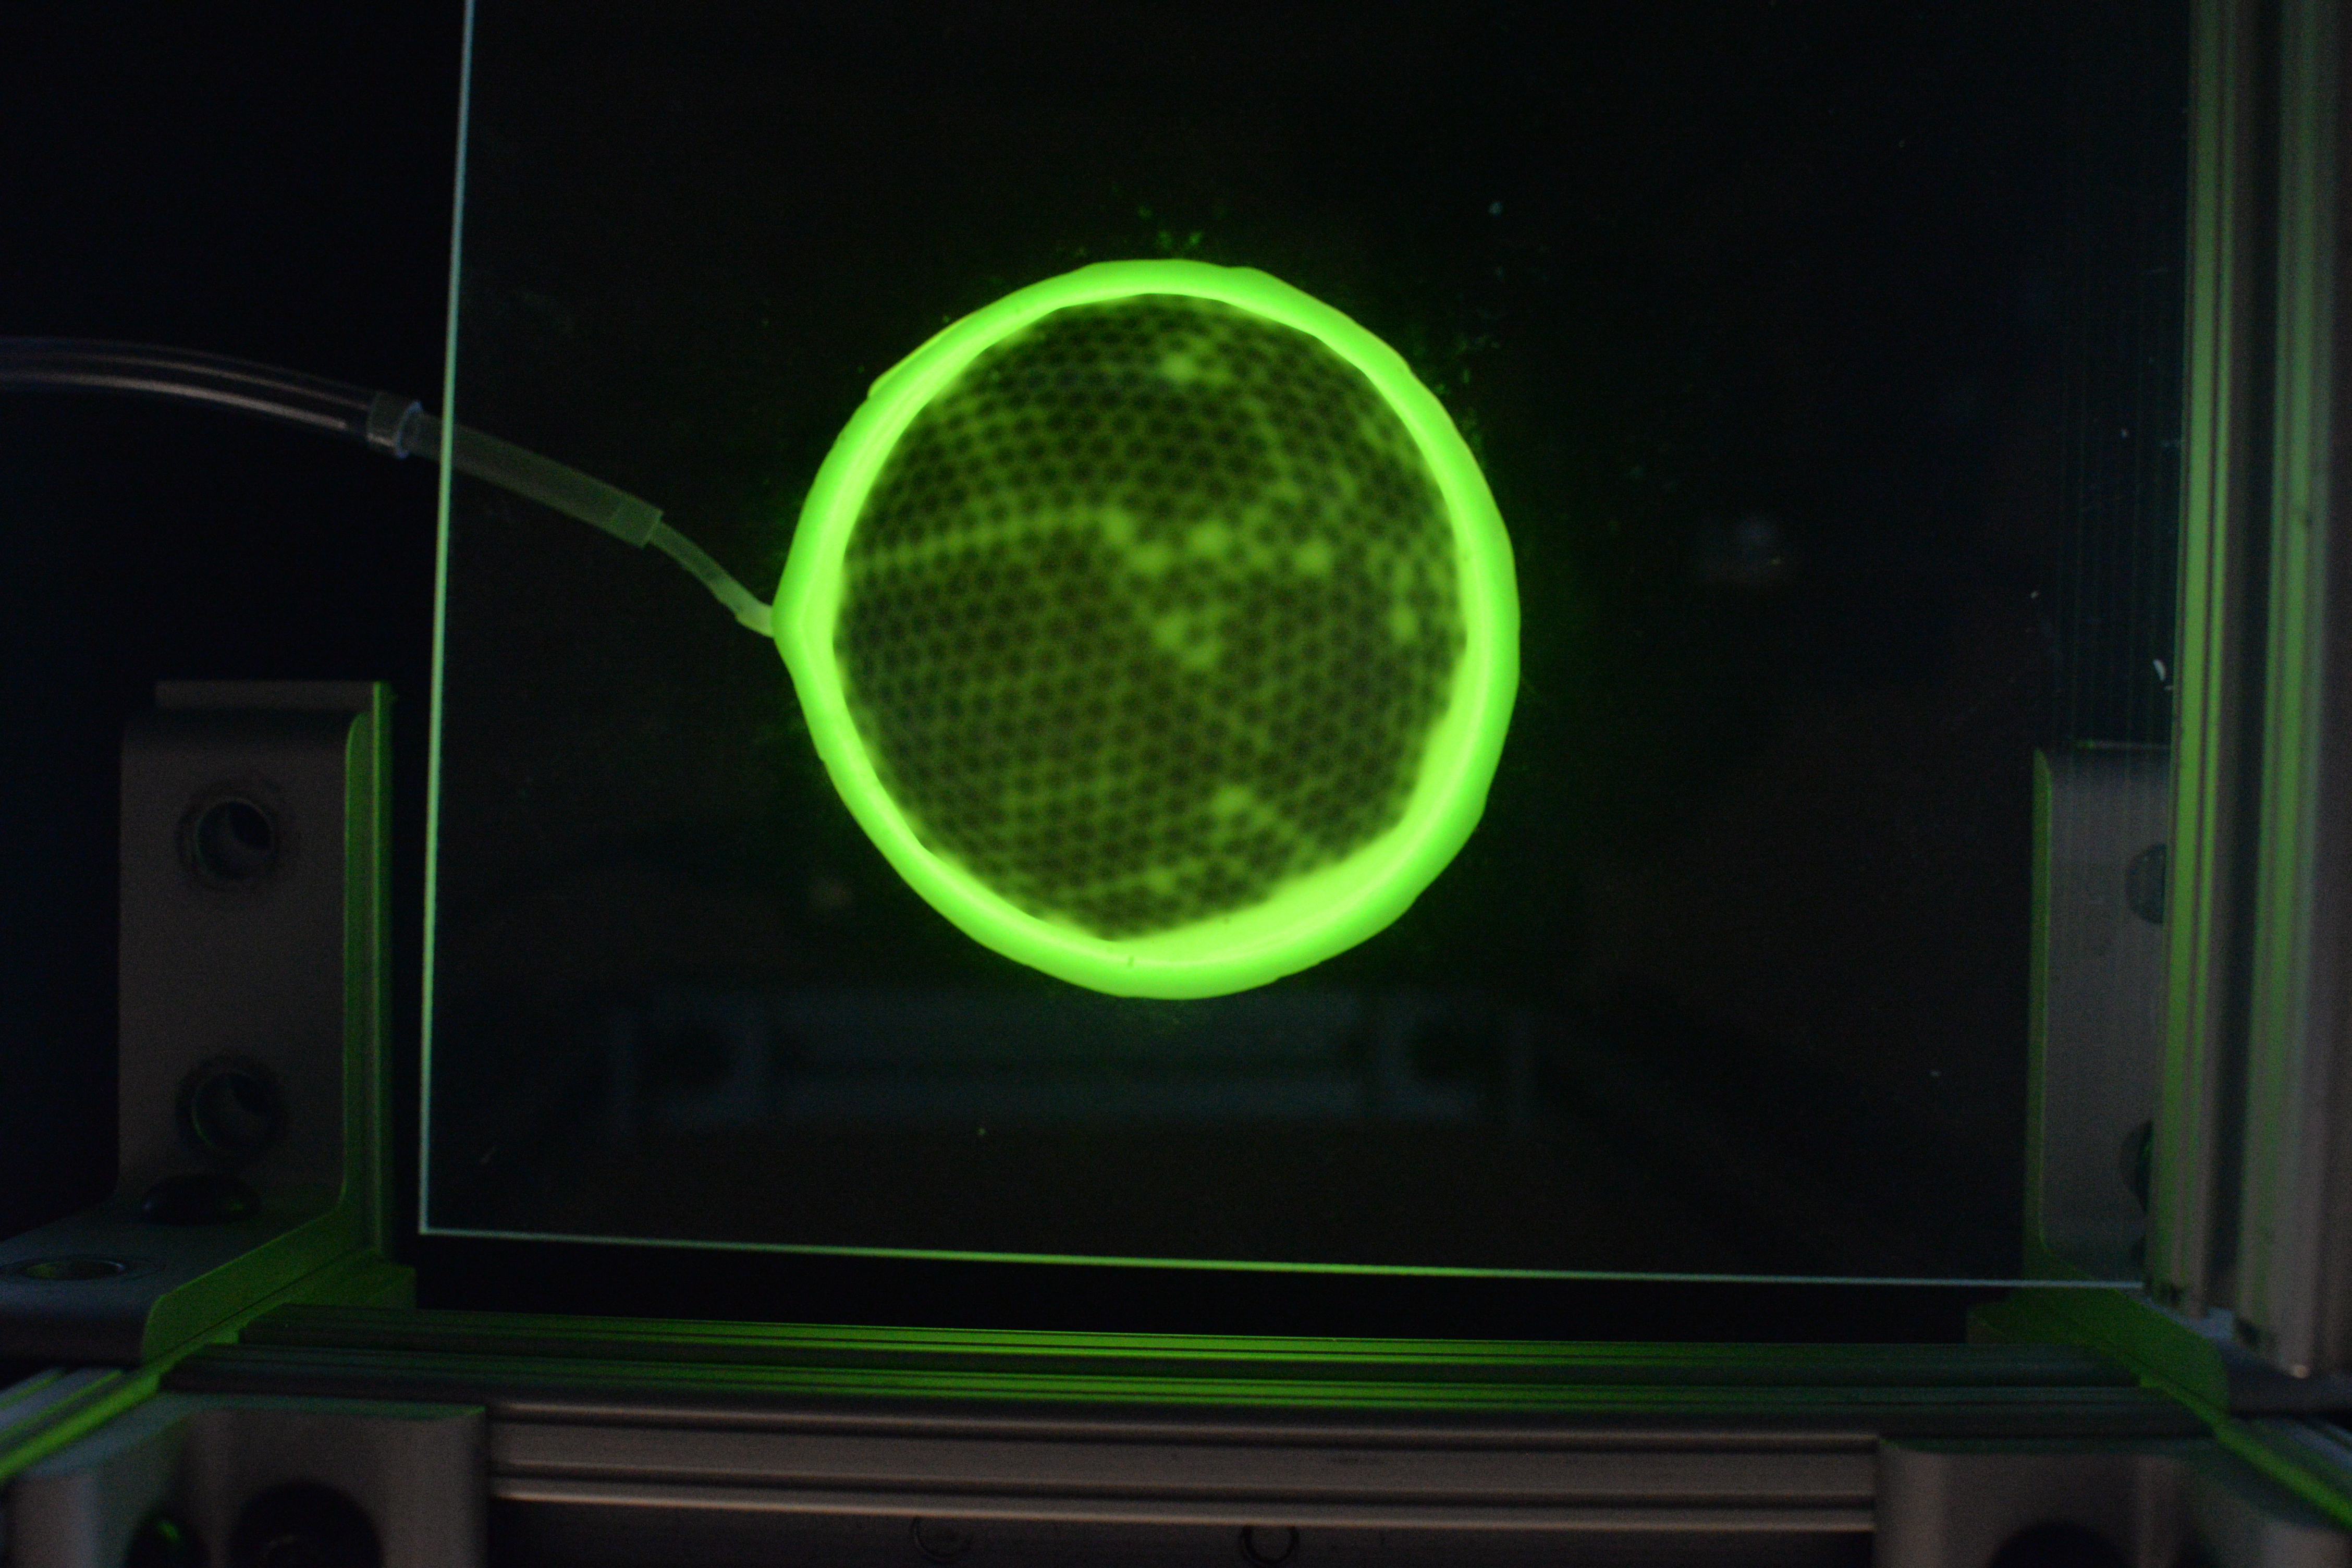
\includegraphics[trim = 345 250 360 95, clip, width=5cm,]{0.423-center}};
		\node[anchor=south west,inner sep=0] at (15,0) {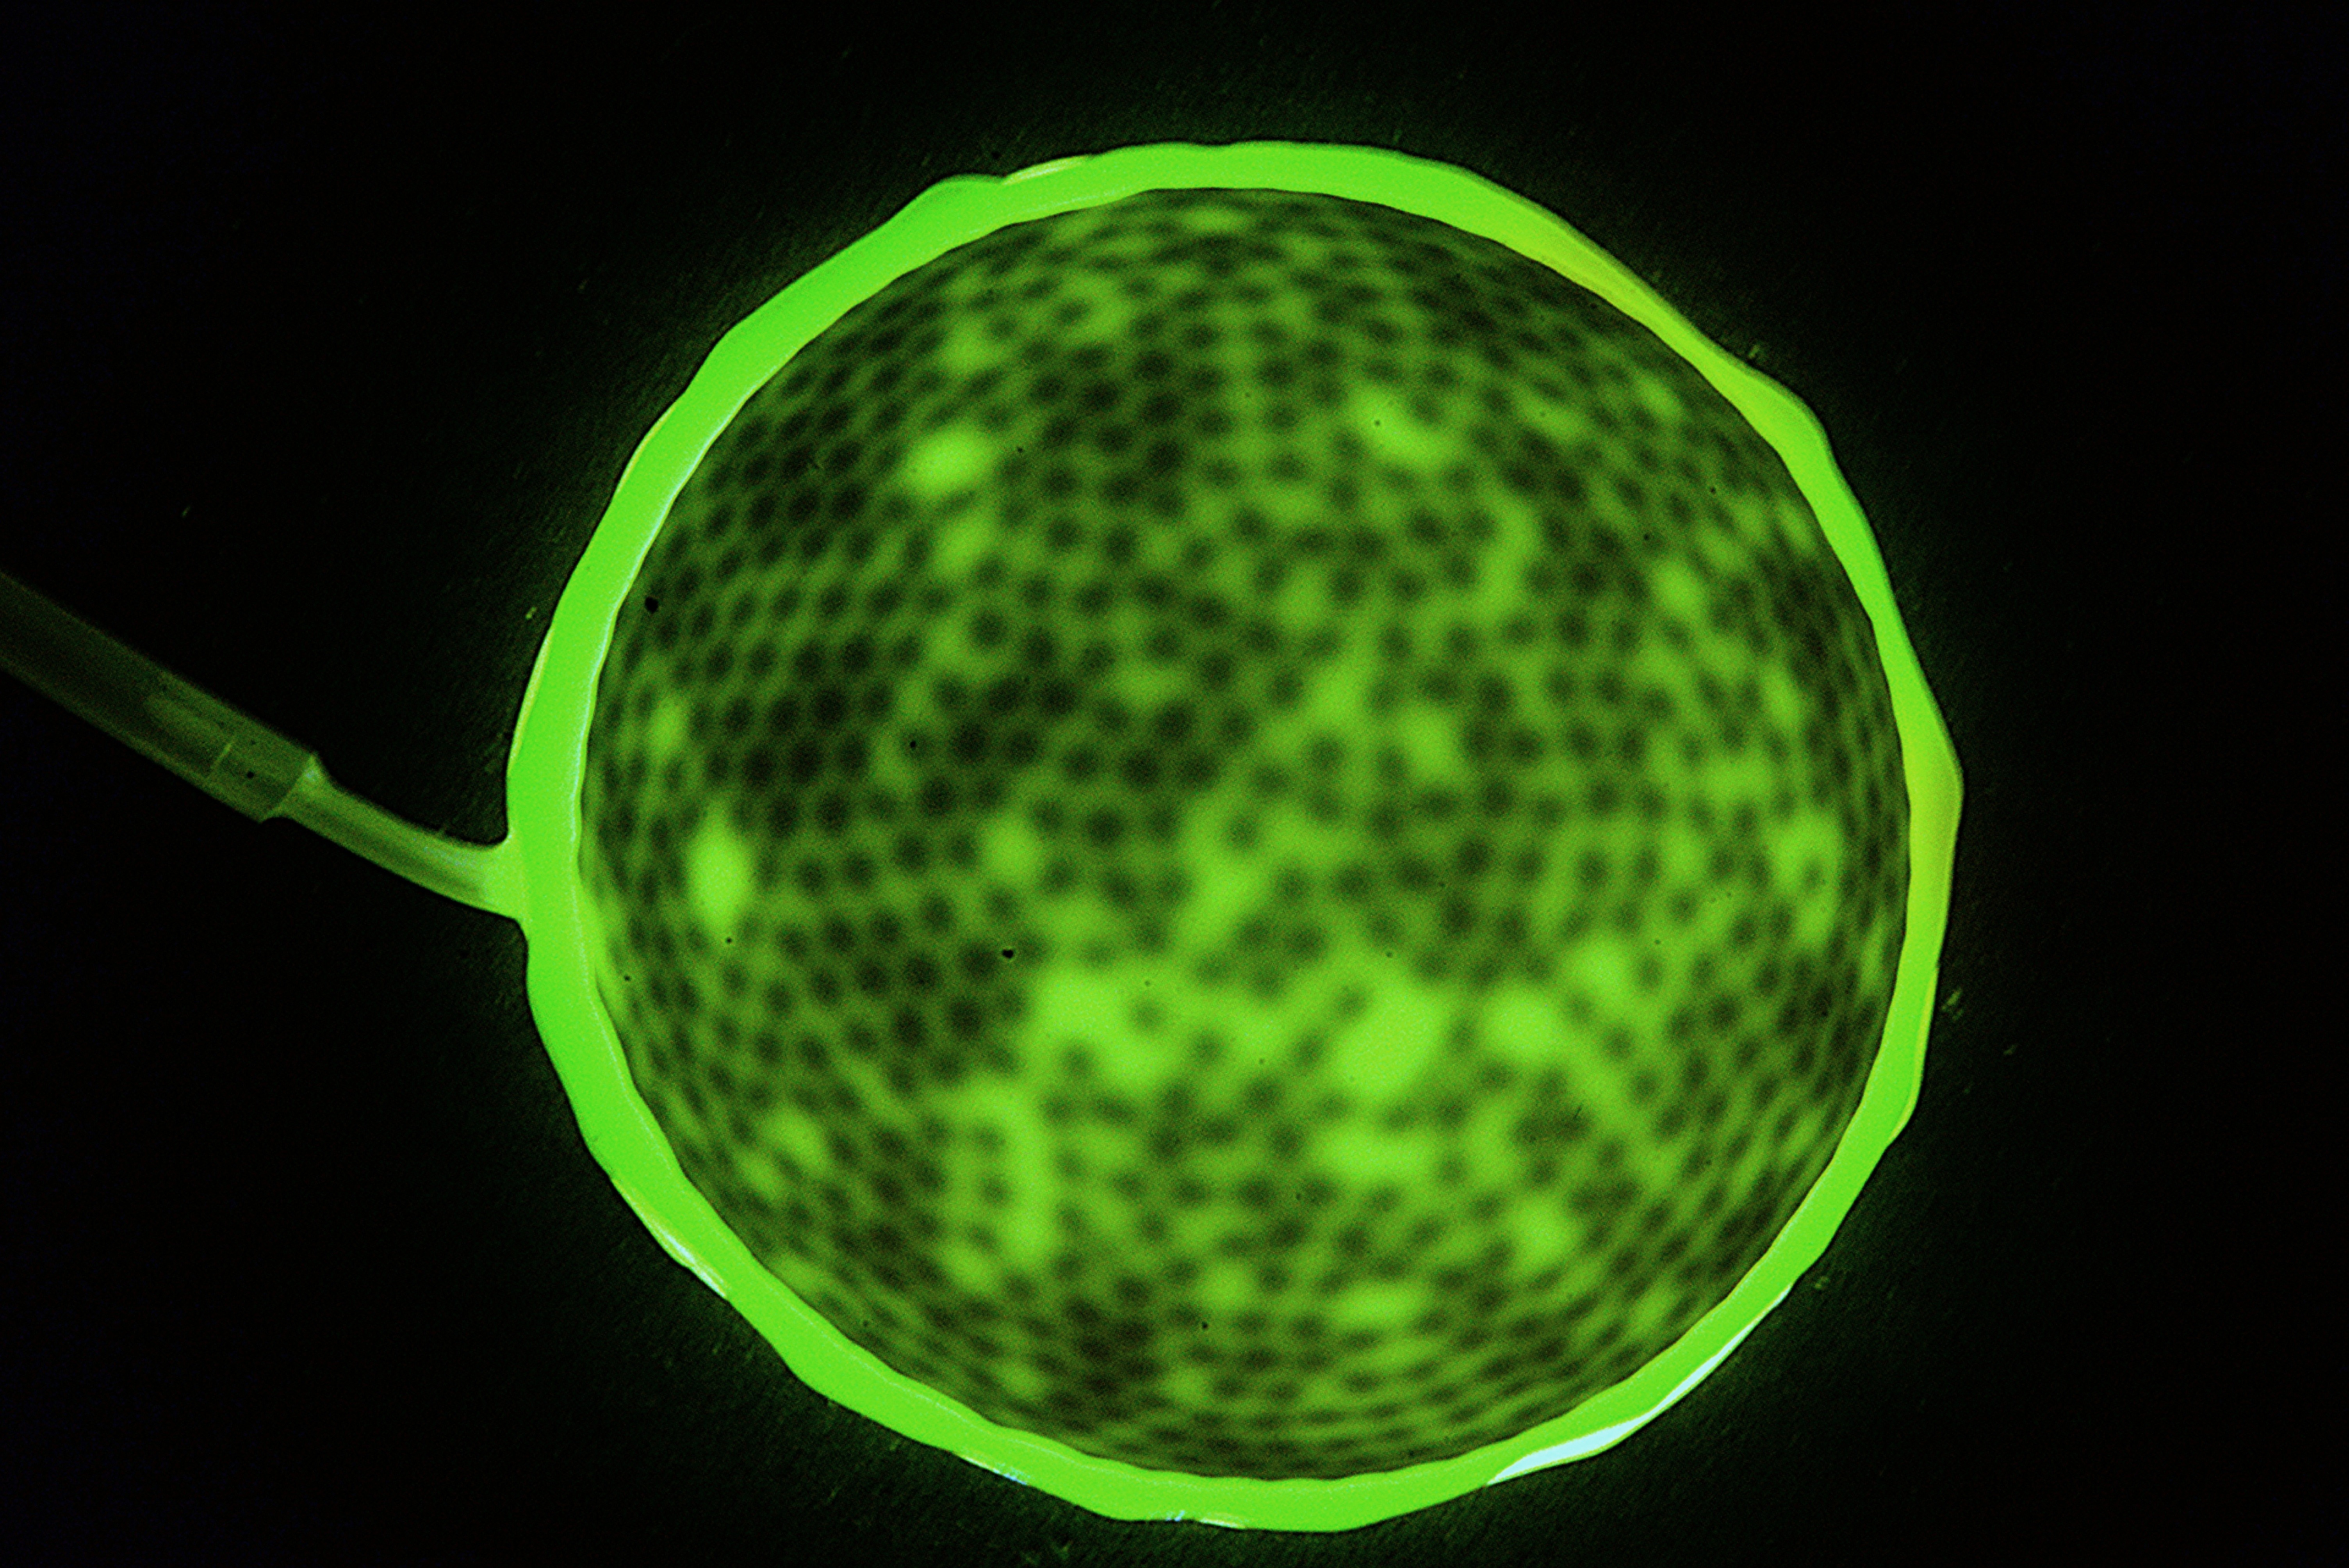
\includegraphics[trim = 1100 0 900 0, clip, width=5cm,]{0.65_1}};
		\node[anchor=south west,inner sep=0] at (20,0) {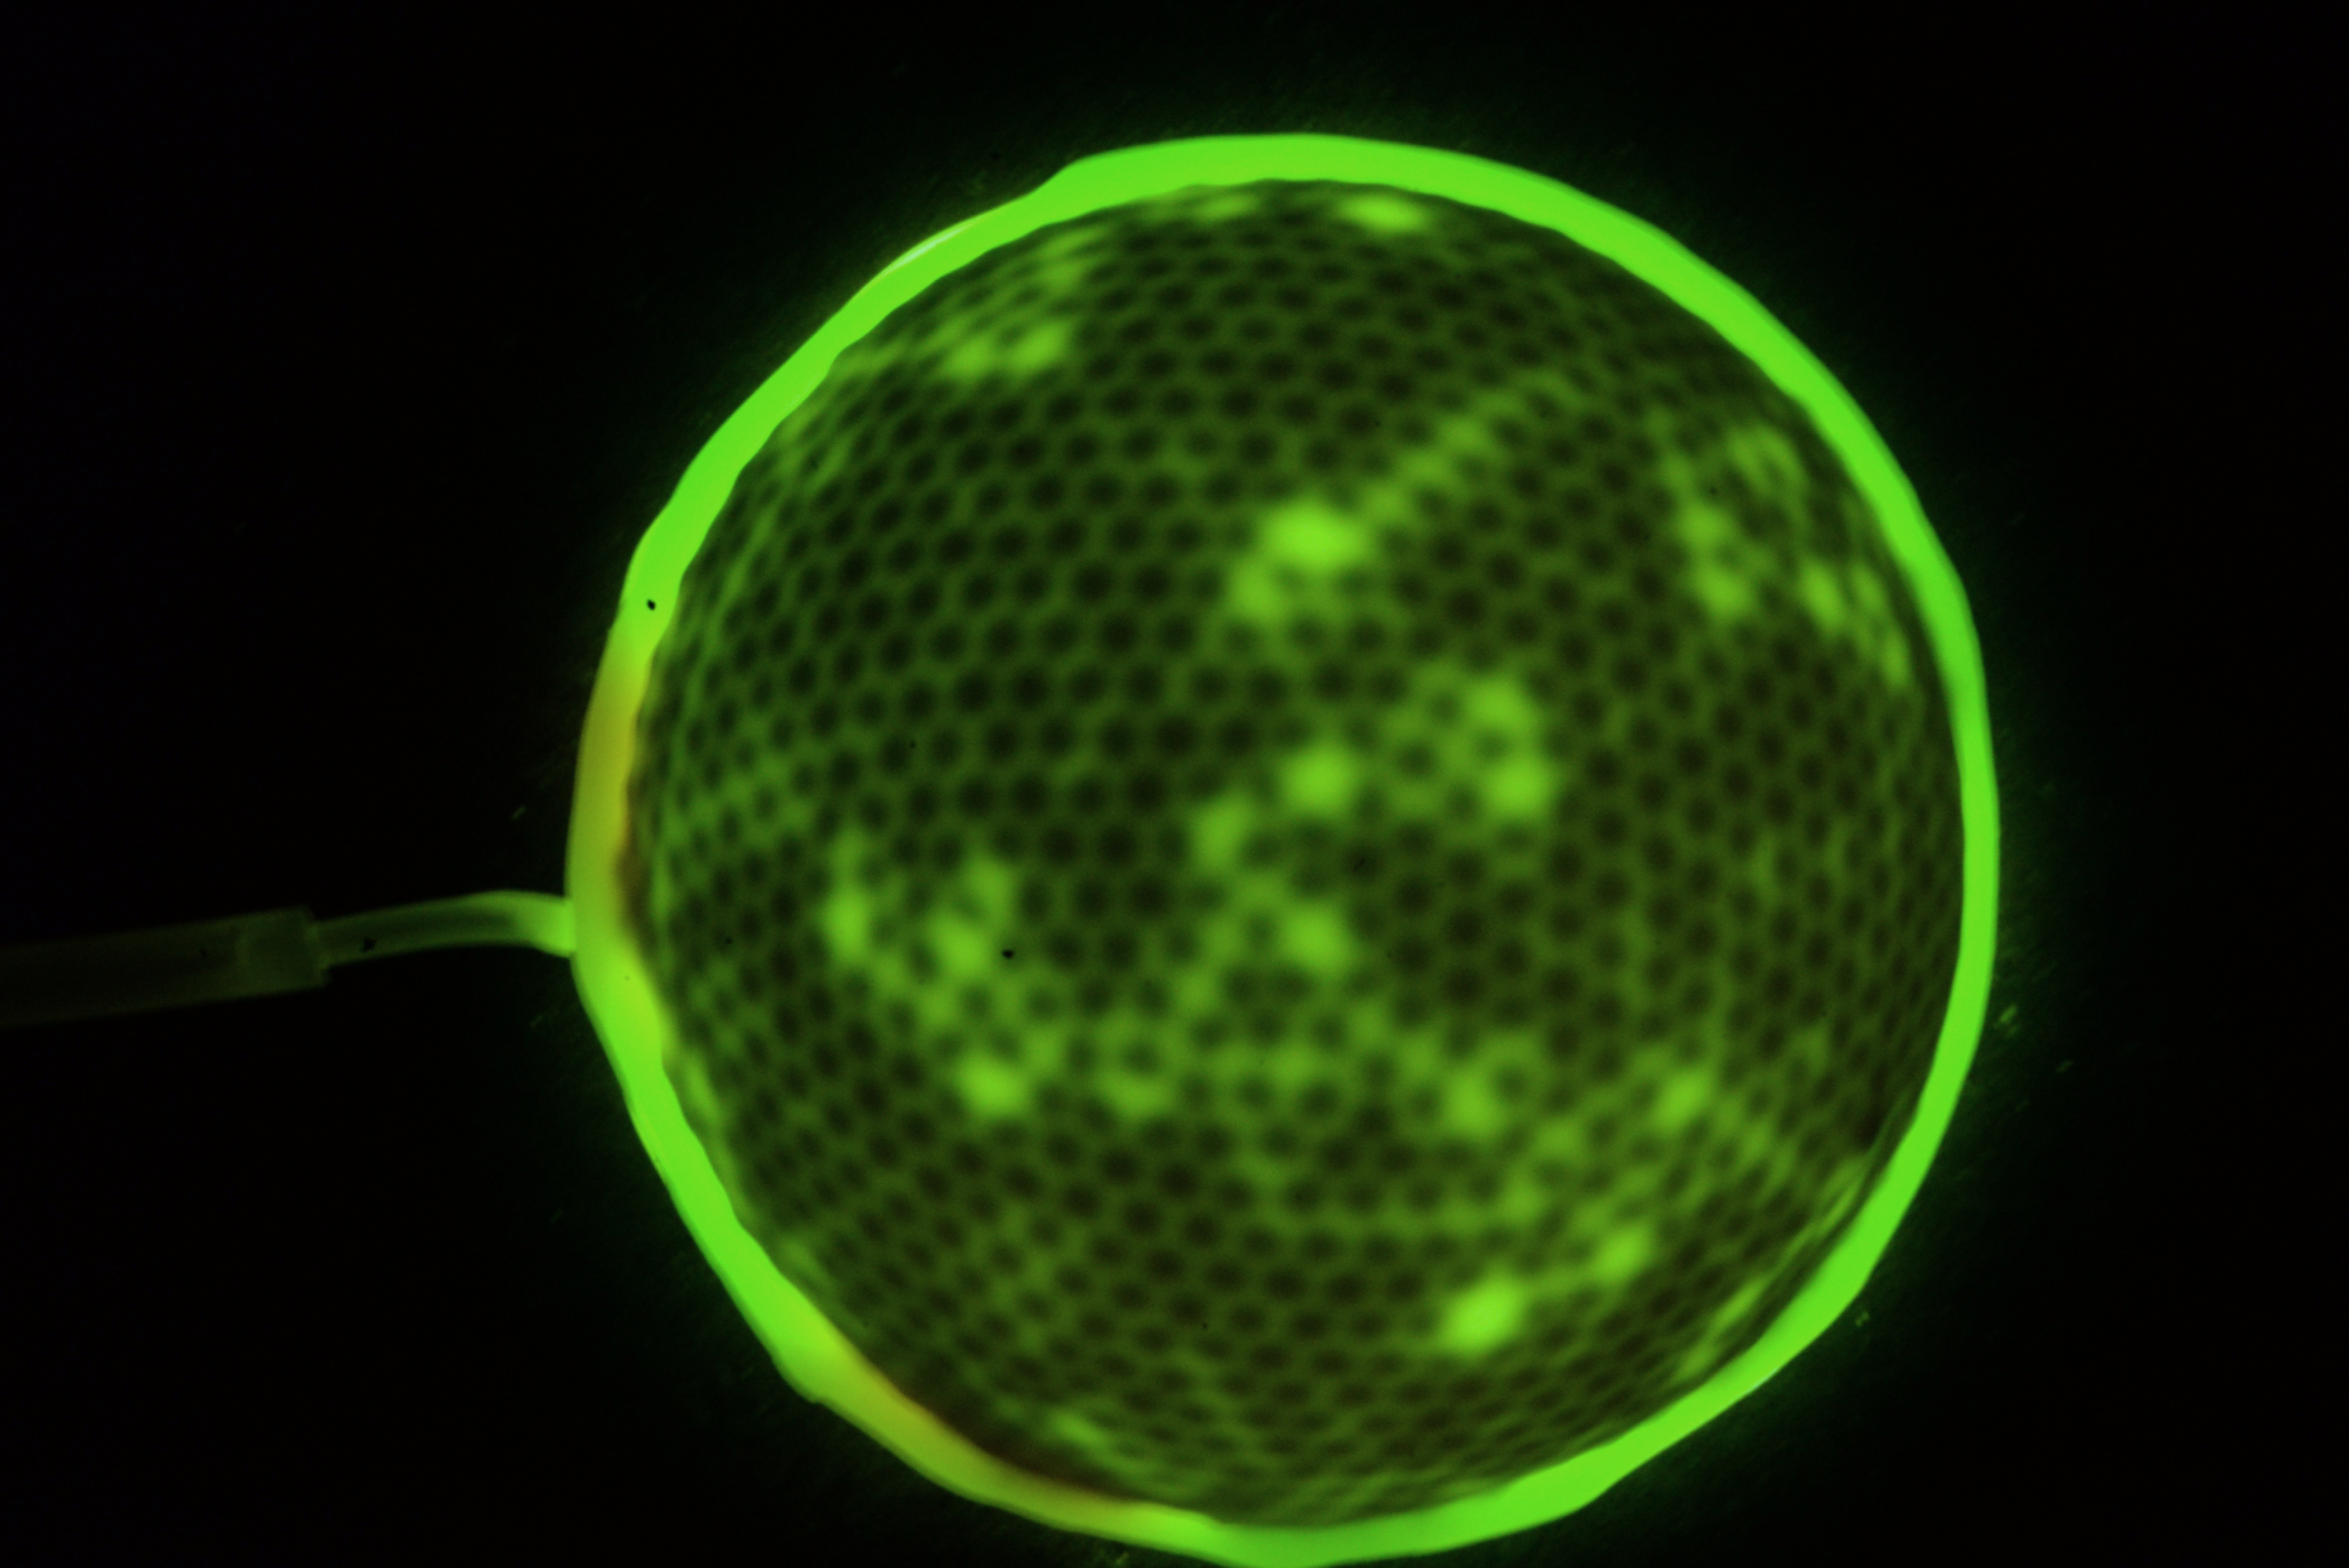
\includegraphics[trim = 1100 0 900 0, clip, width=5cm,]{0.84_1}};
		
		\node [anchor=south west] at (0,4.25) {\color{white}{$i.$}};
		\node [anchor=south west] at (5,4.25) {\color{white}{$ii.$}};
		\node [anchor=south west] at (10,4.25) {\color{white}{$iii.$}};
		\node [anchor=south west] at (15,4.25) {\color{white}{$iv.$}};
		\node [anchor=south west] at (20,4.25) {\color{white}{$v.$}};
		
		%\draw [anchor=south west,black,ultra thick,inner sep=0] (15,4.85) -- (25,4.85) -- (25,0) -- (15,0);
		\draw [anchor=south west,b5,line width=4,inner sep=0] (0,-0.9) -- (0,5.9) -- (15,5.9) -- (15,-0.9) -- (0,-0.9) -- (0,5.9);
		
		%\node [anchor=north] at (2.5,0) {\color{black}{$\phi_0 = 0.44$}};
		\node [anchor=south] at (7.5,5) {\color{black}{$\phi_0 = 0.45$}};
		\node [anchor=north] at (2.5,0) {\color{black}{At Edge}};
		\node [anchor=north] at (7.5,0) {\color{black}{Random}};
		\node [anchor=north] at (12.5,0) {\color{black}{At Apex}};
		\node [anchor=south] at (17.5,5) {\color{black}{$\phi_0 = 0.66$}};
		\node [anchor=south] at (22.5,5) {\color{black}{$\phi_0 = 0.85$}};
		
		%\draw [anchor=north west,blue,ultra thick,inner sep=0] (0,0) -- (5,0);
		
		%\node [anchor=north] at (0,14.35) {\color{black}{{{$p_i =$ 0 kPa, $\delta =$ 0 mm}}}};
		
	\end{tikzpicture}
	
	
\end{document}
